% Estructura Recomendada para Publicación

% Abstract: Mantener actual, es conciso y claro
% Introduction: Agregar párrafo sobre MoE motivation
% Related Work: Muy bueno, mantener
% Problem Formulation: Excelente formalización matemática
% Methodology: Fortalecer con detalles de implementación
% Results: Agregar análisis por patrones de wordlist
% Discussion: Incluir arquitectura MoE propuesta
% Implementation Guidelines: Nueva sección
% Conclusion: Mantener estructura actual



\documentclass[a4paper]{llncs}
\usepackage{amssymb}
\usepackage{graphicx}
\usepackage{url}
\usepackage{xspace}
\usepackage{booktabs}
\usepackage{multirow}
\usepackage{amsmath}
\usepackage{array}

\usepackage{xcolor}
\usepackage{colortbl}
\usepackage{graphicx}

\newcommand{\dga}{\textsc{dga}\xspace}
\newcommand{\moe}{\textsc{moe}\xspace}

\begin{document}

\title{Specialized Expert Models for Wordlist-Based DGA Detection: A Mixture of Experts Approach}

\author{
Reynier Leyva La O \inst{1,2} \and  Rodrigo Gonzalez \inst{1} \and Carlos A. Catania\inst{2}
}

\authorrunning{R. Leyva La O et al.}

\institute{
GridTICs, Facultad Regional Mendoza, Universidad Tecnológica Nacional, Mendoza, Argentina \\ 
\email{rleyvalao@mendoza-conicet.gob.ar }
\and
LABSIN, Facultad de Ingeniería. Universidad Nacional de Cuyo, Mendoza, Argentina \\ \email{harpo@ingenieria.uncuyo.edu.ar}
}

\maketitle

\begin{abstract}


The detection of wordlist-based Domain Generation Algorithms (DGAs) poses a significant challenge for real-time cybersecurity systems, given their semantic coherence and ability to evade traditional heuristics. In this paper, we introduce a systematic methodological framework for selecting expert models within a Mixture of Experts (MoE) architecture, aimed at the efficient and accurate detection of such DGAs.

We conducted an evaluation of seven models on a dataset of 11 DGA families, incorporating a rigorous generalization testing process on families unseen during training. Empirical results identify ModernBERT as the optimal expert model, achieving an F1-score of 86.7\% on known families and 80.9\% on unknown families. Furthermore, this model exhibits an inference time 25× faster than alternatives based on large-scale language models.

Our findings demonstrate that specialized training on the specific domain outperforms general-purpose training strategies, yielding an 8.6\% improvement in F1-score on the training families and a 23.2\% improvement on unseen families. These conclusions establish a set of practical guidelines for deploying scalable and effective MoE-based DGA detection systems in operational environments.



\keywords{Domain Generation Algorithms, Mixture of Experts, Cybersecurity, Real-time Detection, Model Selection}
\end{abstract}


\section{Introduction}
\label{sec:intro}

Domain Generation Algorithms (DGAs) represent a sophisticated evasion technique employed by modern malware to establish resilient Command and Control (C2) communication channels. By deterministically generating thousands of domain names daily, DGAs enable malware families to bypass traditional blacklist-based defenses and maintain persistent operations even when specific domains are discovered and blocked~\cite{plohmann2016comprehensive}.

The cybersecurity landscape has witnessed a concerning evolution toward increasingly sophisticated DGA variants, with wordlist-based algorithms posing the most formidable detection challenges. Unlike conventional DGAs that produce easily identifiable pseudorandom character sequences (e.g., \texttt{qwerty123.com}), wordlist-based variants strategically combine dictionary words and grammatical structures to generate linguistically plausible domains (e.g., \texttt{secure-banking-portal.com}). This semantic coherence enables them to masquerade as legitimate network traffic, rendering traditional entropy-based and character frequency detection methods largely ineffective~\cite{yang2019detecting,Vu2021}.

Current detection methodologies face a fundamental architectural dilemma. Traditional approaches—including character-level CNNs and n-gram analysis—excel at identifying pseudorandom patterns but fail to capture the semantic relationships crucial for wordlist-based detection~\cite{catania2019analysis}. Conversely, sophisticated approaches such as large-scale language models (LLMs) possess the linguistic understanding necessary for semantic pattern recognition but often introduce significant computational overhead that limits their practical deployment. This creates a critical gap between detection capability and operational feasibility, where practitioners must choose between fast but semantically-limited models or accurate but computationally expensive alternatives.

This accuracy-efficiency tension creates a critical deployment barrier in operational cybersecurity contexts. Production networks require systems capable of analyzing DNS traffic with minimal latency while maintaining high detection rates to minimize both false negatives (missed threats) and false positives (operational disruption). Current approaches often force practitioners into suboptimal compromises: deploying fast but semantically-limited models that miss sophisticated threats, or implementing accurate but computationally expensive alternatives that may not scale to high-throughput environments.

The Mixture of Experts (MoE) paradigm offers a principled solution to this dilemma through intelligent computational resource allocation. MoE architectures enable dynamic routing where lightweight models efficiently process routine samples, while specialized expert models are selectively activated for challenging cases requiring sophisticated analysis~\cite{shazeer2017outrageously}. In the context of DGA detection, this translates to using efficient models for clearly malicious pseudorandom domains while reserving computational resources for wordlist-based variants that demand semantic understanding. Such specialization allows each expert to develop focused knowledge on specific threat types, potentially achieving superior performance compared to generalist approaches.

However, realizing MoE's potential for DGA detection requires addressing a fundamental question: \textit{which models should serve as specialized experts for wordlist-based detection?} This selection process must consider multiple competing objectives including detection accuracy, computational efficiency, generalization capability to unseen families, and operational reliability under production constraints. Furthermore, the evaluation must account for the diverse generation strategies employed by different wordlist-based DGA families, from simple concatenation approaches to sophisticated linguistic pattern emulation.

This work addresses the expert selection challenge for wordlist-based DGA detection within MoE architectures through comprehensive empirical analysis. We systematically evaluate seven diverse models ranging from lightweight traditional approaches to state-of-the-art language models, assessing their suitability as specialized experts across multiple performance dimensions. Our evaluation encompasses 11 DGA families with explicit generalization testing on previously unseen families, providing a robust assessment of real-world deployment viability.

While this work is framed within the Mixture of Experts (MoE) paradigm, its scope is explicitly limited to the selection of the most suitable expert model for detecting wordlist-based DGAs. We do not implement a complete MoE architecture with dynamic gating mechanisms or expert coordination in this study. Instead, our focus is on identifying which candidate model offers the best trade-off between detection accuracy, generalization capability, and computational efficiency, with the goal of future integration as a specialized expert in a modular MoE-based system. This targeted scope enables a more rigorous and isolated analysis of semantic detection capabilities, while leaving full MoE system integration as future work.

\textbf{Contributions:} Our primary contributions are:
\begin{enumerate}
    \item[\textbf{(1)}] \textbf{Systematic Evaluation Framework:} We present a comprehensive methodology for evaluating candidate expert models in MoE architectures specifically targeting wordlist-based DGA detection, incorporating both performance and operational constraints.

    \item[\textbf{(2)}] \textbf{Comprehensive Empirical Analysis:} We conduct rigorous evaluation of seven state-of-the-art models across 11 distinct DGA families, including explicit out-of-family generalization testing to assess robustness against emerging threats.

    \item[\textbf{(3)}] \textbf{Composite Performance Metric:} We develop a novel evaluation metric that integrates detection accuracy (precision, recall, F1-score), operational reliability (false positive rate), and deployment feasibility (inference time), enabling holistic model comparison for production deployment.

    \item[\textbf{(4)}] \textbf{Practical Deployment Guidelines:} We provide actionable recommendations for expert selection in production MoE systems, including identification of optimal models and characterization of their strengths and limitations across different DGA variants.

    \item[\textbf{(5)}] \textbf{Performance Characterization:} We identify ModernBERT as the optimal expert for wordlist-based detection, achieving 86.7\% F1-score with 26ms inference time, while revealing persistent challenges with sophisticated families like \textit{manuelita} that require specialized approaches.
\end{enumerate}

These contributions establish a foundation for practical MoE deployment in cybersecurity contexts, enabling systems that maintain both detection effectiveness and operational efficiency under real-world constraints.





\section{Related Work}
\label{sec:Related work}

\subsection{Detection Challenges in Wordlist-Based DGAs}

Wordlist-based DGAs generate syntactically plausible and semantically coherent domain names (e.g., \texttt{secure-login-check.com}), which evade entropy-based heuristics and character-distribution models commonly used in classical DGA detection approaches. This category of DGAs poses a significant challenge due to the lack of obvious statistical irregularities and their high similarity to legitimate domains \cite{plohmann2016comprehensive,cebere2024down}. While arithmetic and hash-based DGAs are easily detected due to their randomness and unnatural patterns, wordlist-based DGAs blend into benign DNS traffic, often producing high false-positive rates \cite{yu2018character}.

\subsection{Limitations in Existing Detection Literature}

Recent surveys \cite{cebere2024down} have revealed that many detection models are evaluated under idealized conditions that do not reflect real-world deployment. Cebere et al.\ analyze 38 contextless detection papers and identify recurring assumptions that undermine the generalizability and robustness of many proposed solutions. Among the most critical findings:

\begin{itemize}
    
    \item \textbf{Dataset Bias:} Most prior work evaluates models on easy-to-detect families (e.g., arithmetic or hash-based DGAs), while more difficult families—particularly wordlist-based and adversarial—are underrepresented. This bias leads to inflated accuracy metrics that do not translate to operational settings \cite{cebere2024down}.
    
    \item \textbf{Generalization Failure:} Models trained on specific families often fail to generalize to unseen DGAs. The same study shows that performance degrades significantly on novel families, with F1-scores for wordlist DGAs frequently below 0.7 \cite{cebere2024down}.
    
    \item \textbf{Assumption of Maliciousness:} Binary classifiers typically assume that all AGDs are malicious, overlooking benign uses of DGAs (e.g., DNS benchmarking tools), which can lead to false positives \cite{antonakakis2012throw}.

    \item \textbf{Lack of Reproducibility:} Most prior work does not release model implementations or trained weights, hindering fair comparisons and real-world deployment testing. Only a few recent studies (e.g., \cite{cebere2024down}) provide open-source benchmarks covering a broad range of DGA families, enabling reproducibility and transparent evaluation.
    
\end{itemize}

\subsection{Detection Architectures in the Literature}

Table~2 in \cite{cebere2024down} summarizes over 30 DGA detection models across multiple architectures, including Random Forests, RNNs, CNNs, ResNets, and Transformer-based approaches. While deep learning methods dominate recent literature, their practical applicability remains limited by factors such as inference latency and training data requirements.

Notably, only a few models are tailored to detect stealthy DGAs like wordlist-based families (e.g., Suppobox, Matsnu). These families occupy distributional regions close to legitimate domains (as shown by t-SNE projections in \cite{cebere2024down}), demanding semantically-aware models rather than pure statistical or character-level approaches.

\subsection{Our Contribution}

In response to these gaps, our work proposes a mixture of expert classifiers specializing in different DGA families, with a particular focus on wordlist-based variants. We adhere to the recommendations of \cite{cebere2024down}, adopting realistic assumptions, diverse families (including challenging ones), and evaluating multiclass setups that distinguish between benign and malicious generators.

Our approach offers both interpretability and modularity, enabling precise attribution of detected domains to specific DGA families. This is essential not only for threat intelligence but also for reducing false positives in benign-but-algorithmic domain usage.

To promote reproducibility and facilitate future research, we release the full source code, pretrained models, and the complete experimental dataset used in our study. This contrasts with the majority of prior work, which often fails to publish either code or trained weights \cite{cebere2024down}, hindering comparative evaluation and real-world validation.



\section{Problem Formulation}

The core challenge addressed in this work is the \textbf{selection of an optimal specialized expert model} for detecting \textbf{wordlist-based DGAs} within a \textit{MoE} architecture.

In MoE-based DGA detection systems, it is beneficial to assign \textit{dedicated expert models to different DGA subfamilies}, particularly when those subfamilies differ significantly in their structural and semantic characteristics. Among these, \textbf{wordlist-based DGAs present the greatest challenge}, as they generate syntactically coherent and linguistically plausible domain names that closely resemble legitimate traffic, making them difficult to detect using traditional methods.

Our objective is to \textbf{identify the best-performing expert model for robust detection of wordlist-based DGAs}, while simultaneously balancing \textit{detection precision}, \textit{generalization capability}, and \textit{computational efficiency}. The selected model is intended to act as a \textbf{specialized expert} within a broader MoE framework, where simpler models are responsible for detecting more easily identifiable DGA types.

\textbf{Evaluation Metrics.} To guide expert model selection, we define a composite scoring function that integrates commonly used classification metrics. Table~\ref{tab:metrics} presents the specific formulas used to calculate each metric.

\begin{table}[h]
\centering
\caption{Evaluation metrics used for expert selection}
\label{tab:metrics}
\small % Reduce font size for the whole table
\renewcommand{\arraystretch}{1.5} % Add vertical space between rows
\begin{tabular}{ll}
\toprule
\textbf{Metric} & \textbf{Formula} \\
\midrule
Precision & $\textstyle \frac{TP}{TP + FP}$ \\
Recall  & $\textstyle \frac{TP}{TP + FN}$ \\
F1 Score & $\textstyle 2 \cdot \frac{\text{Precision} \cdot \text{Recall}}{\text{Precision} + \text{Recall}}$ \\
False Positive Rate (FPR) & $\textstyle \frac{FP}{FP + TN}$ \\
\bottomrule
\end{tabular}
\end{table}



\textbf{Composite Model Selection Function.} Let $E = \{E_1, E_2, \ldots, E_n\}$ denote the set of candidate models evaluated on a dataset $D$ that includes both benign domains and samples from multiple wordlist-based DGA families. We define the optimal expert model $E^*$ as the one that maximizes the following objective function:

\begin{equation}
E^* = \arg\max_{E_i \in E} f(F1_i, P_i, R_i, T_i, FPR_i)
\end{equation}

where:
\begin{itemize}
    \item $F1_i$: F1-score of model $E_i$
    \item $P_i$: Precision
    \item $R_i$: Recall
    \item $FPR_i$: False positive rate
    \item $T_i$: Inference time (latency)
\end{itemize}

The scoring function $f(\cdot)$ integrates these metrics with equal weights to balance detection performance and real-time applicability:

\begin{equation}
f(\cdot) = \alpha \cdot F1 + \beta \cdot (1 - FPR) + \gamma \cdot P + \delta \cdot R + \epsilon \cdot \left(1 - \frac{T}{T_{\text{max}}}\right)
\end{equation}

where $\alpha = \beta = \gamma = \delta = \epsilon = 0.2$ by default, although these weights may be tuned depending on deployment requirements.

This formulation allows us to \textit{holistically rank} the candidate models by simultaneously considering their \textbf{detection capability for linguistically complex threats} and their \textbf{practical feasibility in real-time cybersecurity environments}. The model achieving the highest composite score is selected as the \textbf{wordlist-based expert} in the MoE system, complementing other experts to effectively cover the diverse landscape of DGA variants.





\section{Methodology}
\label{sec:methodology}

To identify the optimal specialized expert for detecting wordlist-based DGAs in a MoE architecture, we designed a comprehensive evaluation methodology covering dataset construction, model selection, and performance assessment under realistic deployment constraints.

\subsection{Dataset Construction and Characteristics}
\label{subsec:dataset}
We constructed a balanced dataset that reflects realistic network traffic conditions and encompasses the diverse generation patterns of wordlist-based DGAs. The dataset was divided as follows:

\begin{table}[h]
\centering
\caption{Detailed composition of the dataset used for model training and evaluation. The table lists the wordlist-based DGA families used for training and generalization testing, along with the corresponding number of samples. Legitimate domains were included to simulate real network traffic and were split into training and testing subsets accordingly.}
\label{tab:dataset_composition}
\resizebox{0.7\textwidth}{!}{%
\begin{tabular}{l|c|c|c}
\toprule
\textbf{Category} & \textbf{Family Name} & \textbf{Training Samples} & \textbf{Test Samples} \\
\midrule
\multirow{8}{*}{\textbf{Training Families}} 
& charbot     & 10,000 & 3,000 \\
& deception   & 10,000 & 3,000 \\
& gozi        & 10,000 & 3,000 \\
& manuelita   & 10,000 & 3,000 \\
& matsnu      & 10,000 & 3,000 \\
& nymaim      & 10,000 & 3,000 \\
& rovnix      & 10,000 & 3,000 \\
& suppobox    & 10,000 & 3,000 \\
\midrule
\multirow{3}{*}{\textbf{Generalization Families}} 
& bigviktor   & --     & 3,000 \\
& ngioweb     & --     & 3,000 \\
& pizd        & --     & 3,000 \\
\midrule
\textbf{Legitimate Domains} & - & 80,000 & 6,000 \\
\bottomrule
\end{tabular}
}
\end{table}

DGA domains were sourced from established public repositories, including DGArchive~\cite{plohmann2015dgaarchive}, 360 Netlab~\cite{360netlab}, and UMUDga~\cite{zago2020umudga}. Where necessary, domains were regenerated using family-specific code, including the \textit{charbot} generator~\cite{peck2019charbot}, ensuring temporal and structural diversity.

Legitimate domains were sampled from the Tranco top sites list, reflecting benign traffic typically observed in real-world DNS datasets \cite{tranco}.

This dataset captures diverse wordlist-based generation strategies, from basic concatenation to advanced semantic mimicry, ensuring a comprehensive evaluation landscape.


\subsection{Model Selection and Architecture Diversity}

We selected seven models representing a broad spectrum of architectural paradigms and deployment costs, ensuring comprehensive evaluation across both accuracy and efficiency dimensions.

\begin{itemize}
    \item \textbf{Large Language Models (LLMs)}: \textit{Gemma 3 4B} \cite{gemma_docs_2024,gemma3-4b-it} and \textit{LLaMA 3.2 3B} \cite{llama3_hf_2024} offer strong semantic representation capabilities but come with high inference cost \cite{la2024llms,sayed2024fine}.
    \item \textbf{Specialized Transformers}: \textit{ModernBERT} \cite{modernbert_hf_2024}, a production-optimized BERT variant, and \textit{DomBertUrl} \cite{mahdaouy2024domurls_bert}, pre-trained on domain/URL data, provide a trade-off between linguistic modeling and computational efficiency.
    \item \textbf{Traditional Approaches}: \textit{CNN} (character-level) \cite{catania2019analysis}, \textit{Random Forest} (feature-based baseline) \cite{Vu2021}, and \textit{LA\_Bin07} (lexical analysis-based) represent lightweight models with proven utility in fast, high-throughput settings \cite{tuan2022detecting}.
\end{itemize}

This selection allows for comparing models not only based on their raw detection performance, but also on other characteristics such as semantic understanding and inference speed.






\subsection{Training and Evaluation Framework}
All experiments were conducted in a standardized environment using an NVIDIA Tesla T4 GPU on Google Colab \cite{google_colab}. This setup ensured consistent hardware performance across both training and evaluation phases for all models.

\textbf{Training Setup.} Our training methodology follows a systematic approach to ensure fair model comparison, as illustrated in Figure~\ref{fig:training_phase}. We constructed a balanced dataset composed of eight carefully selected DGA families for training, with each family contributing exactly 10,000 malicious domains, totaling 80,000 DGA domains. To reflect realistic network traffic conditions and maintain class balance, we included an additional 80,000 benign domains sourced from legitimate web traffic. This results in a comprehensive 160K domain training set with a 50-50 distribution between malicious and benign samples. Further details on dataset construction and family selection criteria are provided in Section~\ref{subsec:dataset}. 

All models were trained independently on this identical dataset to ensure a fair comparison of learning capabilities across different architectural paradigms. The standardized training environment, combined with consistent hardware allocation, eliminates potential confounding factors that could bias performance comparisons.

\textbf{Evaluation Procedure.} Our evaluation framework implements a rigorous two-stage strategy designed to assess both memorization capabilities and generalization performance, as detailed in Figure~\ref{fig:evaluation_phase}. The framework consists of: (i) in-family evaluation measuring performance on DGA families seen during training, and (ii) generalization evaluation testing robustness against previously unseen families.

For the in-family evaluation, we tested each model using 1,500 DGA domains sampled from each of the eight training families. Crucially, these domains were combined with the same set of 1,500 benign domains across all families, creating a controlled experimental design that isolates the effect of different DGA generation strategies while maintaining consistent benign traffic patterns. This approach resulted in 3,000 total domains per family, from which we constructed 30 independent batches of 100 domains each (50 benign and 50 malicious). This batch-based design serves dual purposes: it simulates real-world streaming scenarios where classification must remain consistent under varying input conditions, and it enables robust statistical analysis through repeated sampling.

For the generalization evaluation, we employed three DGA families that were completely excluded from the training phase. Each family was paired with a different set of 1,500 benign domains, with each benign set remaining fixed across its respective family. This experimental design isolates the effect of changes in malicious domain structure while avoiding confounding due to variation in benign traffic characteristics. The same batch construction methodology was applied, resulting in 30 batches per generalization family.

This evaluation strategy fundamentally relies on repeated sampling principles, with each family assessed through 30 randomly constructed batches. This approach enables statistically robust estimates of performance metrics and provides confidence intervals for model comparison, following the established principles of sampling theory described by Cochran~\cite{cochran1977sampling}. The resulting framework allows us to compute mean and standard deviation for key metrics including precision, recall, F1-score, and false positive rate, providing comprehensive performance characterization under realistic deployment conditions.

\begin{figure}[ht]
    \centering
    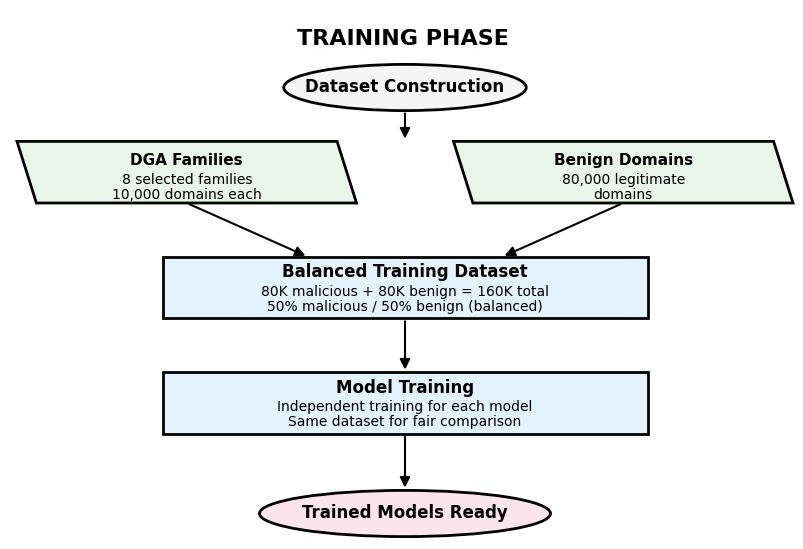
\includegraphics[width=0.85\textwidth]{Train.jpg}
    \caption{Training phase workflow showing the systematic construction of a balanced dataset from 8 selected DGA families (10,000 domains each) combined with 80,000 benign domains, resulting in a 160K domain training set. The diagram illustrates the standardized training protocol ensuring fair model comparison under consistent hardware conditions (NVIDIA Tesla T4 GPU, Google Colab).}
    \label{fig:training_phase}
\end{figure}

\begin{figure}[ht]
    \centering
    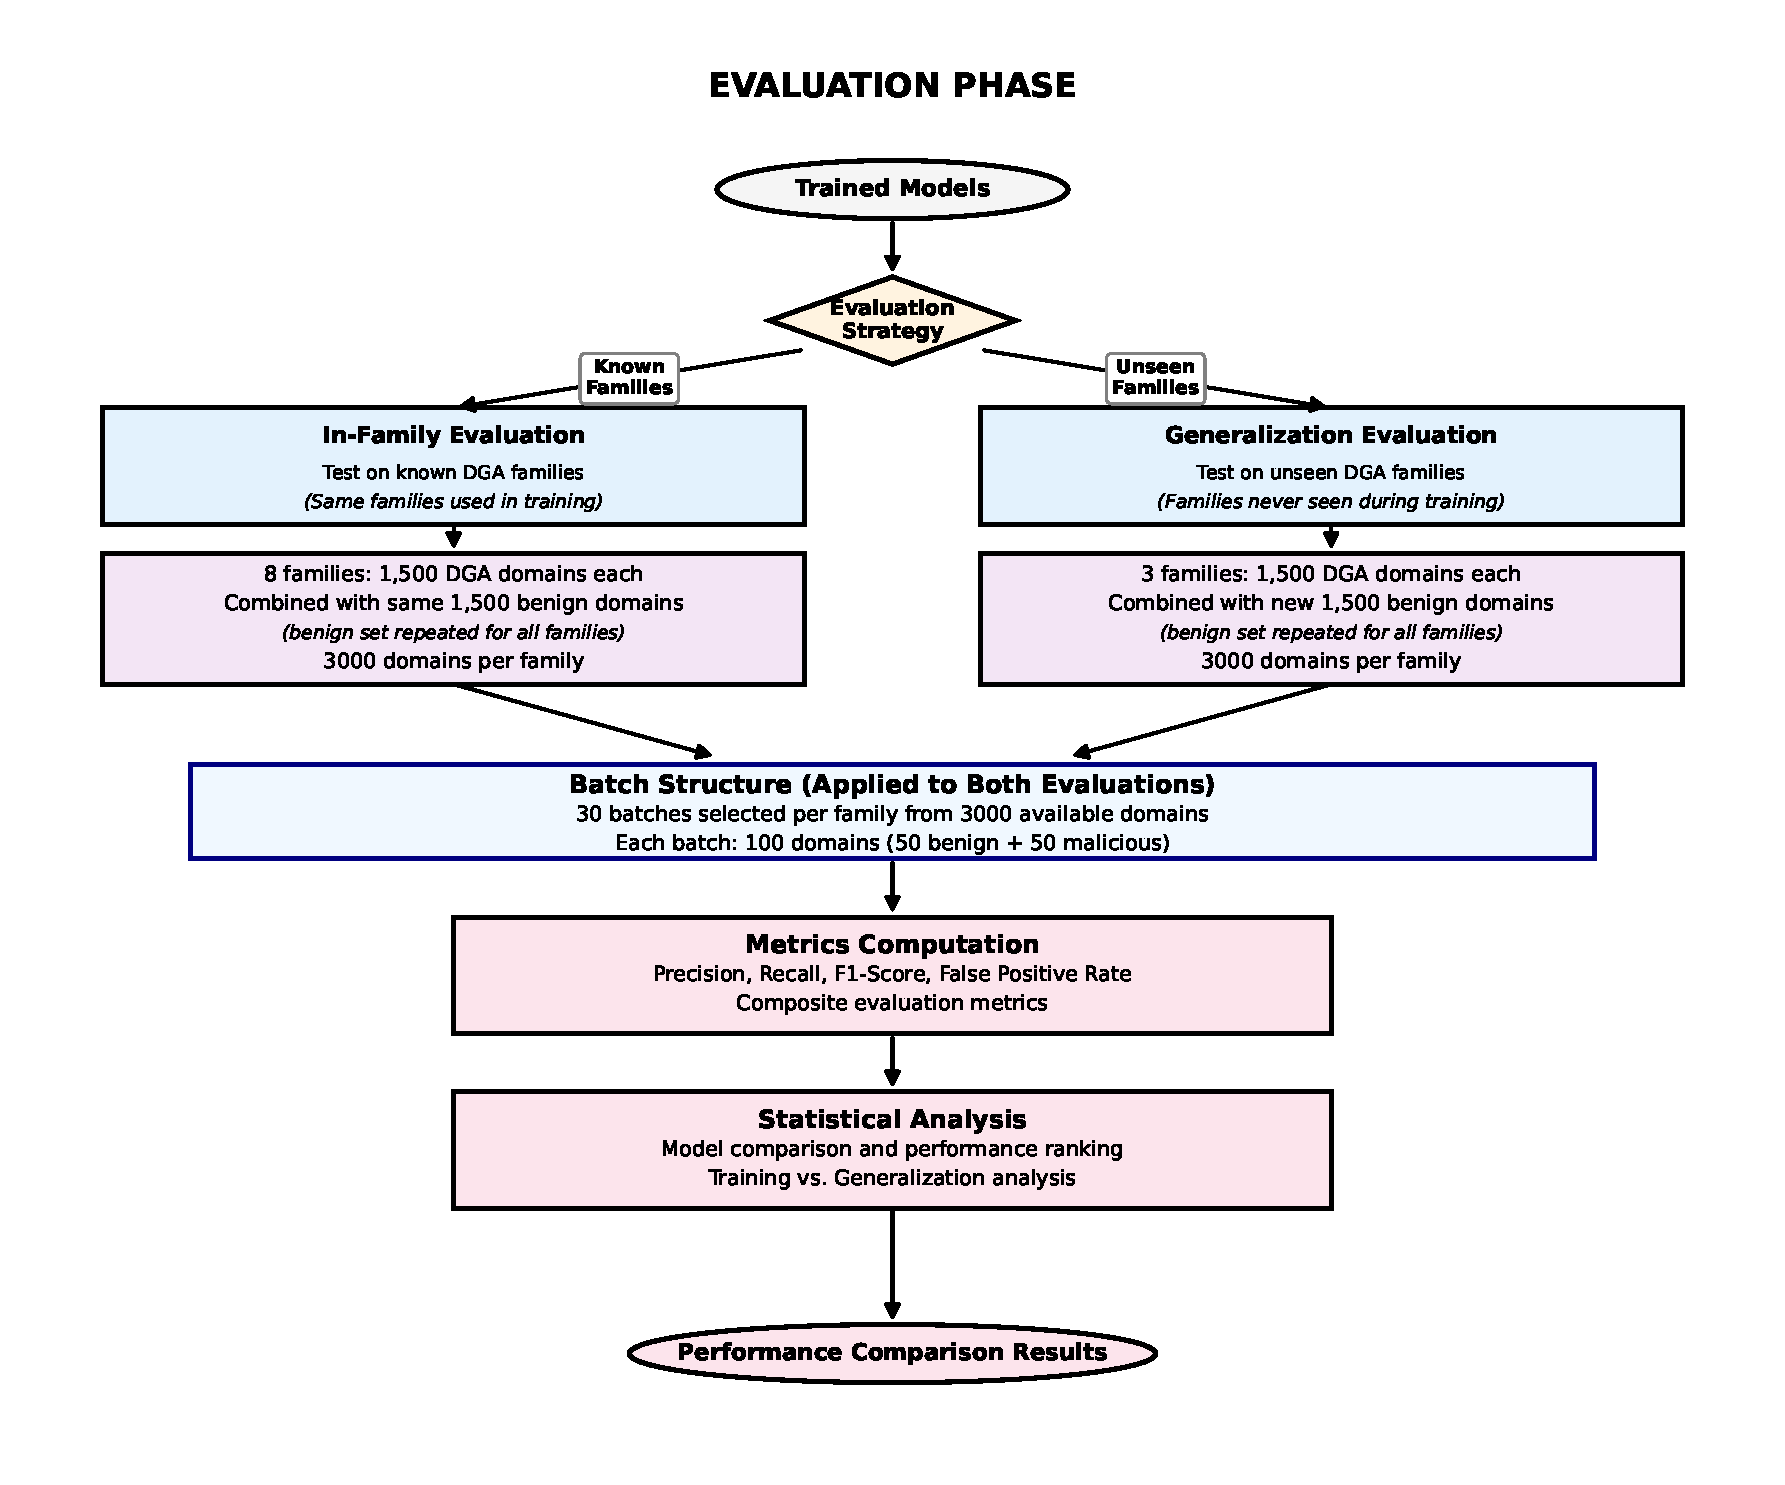
\includegraphics[width=\textwidth]{evaluation_phase.pdf}
    \caption{Evaluation phase workflow detailing the two-stage assessment strategy. The framework implements: (1) In-family evaluation using 8 known DGA families with controlled benign sets to assess memorization capabilities, and (2) Generalization evaluation using 3 unseen DGA families with unique benign sets to test robustness. Both strategies employ 30 randomly sampled batches of 100 domains (50+50) per family, enabling statistical analysis through repeated sampling and providing robust performance estimates.}
    \label{fig:evaluation_phase}
\end{figure}


\subsection{Extended Evaluation: Multi-Family Training Comparison}

To further validate our expert selection findings, we conduct an additional comparative evaluation where the optimal selected expert is trained using an expanded dataset encompassing 54 DGA families, following the methodology established by La O et al. \cite{la2024llms}. This extended training set includes the 8 wordlist-based families used in our primary evaluation plus 46 additional DGA families representing diverse generation strategies (algorithmic, hash-based, and hybrid approaches).

The purpose of this comparison is to investigate whether specialization on wordlist-based DGAs (our 8-family expert) provides advantages over a generalist approach trained on a broader spectrum of DGA types. This evaluation addresses a critical question for MoE deployment: whether expert specialization outperforms general-purpose models with broader training exposure.

The multi-family trained model uses identical architecture and hyperparameters as our specialized expert, with the only difference being the training data composition. Both models are evaluated using the same test sets to ensure fair comparison.


\section{Experimental Results}
\label{sec:results}

\subsection{Overall Performance Analysis}

Our comprehensive evaluation of seven models reveals substantial performance differences, which directly impact the selection of a specialized expert for MoE architectures. Table~\ref{tab:individual-performance} summarizes key metrics for both training and generalization scenarios.

\begin{table}[ht]
\centering
\caption{Performance comparison of candidate expert models on wordlist-based DGA detection. Training reflects results on 8 known families, while generalization tests robustness on 3 unseen families. The composite score integrates accuracy, efficiency, and reliability.}
\label{tab:individual-performance}
\resizebox{0.6\textwidth}{!}{%
\begin{tabular}{l|c|c|c|c|c|c}
\toprule
\textbf{Model} & \textbf{Prec.} & \textbf{Recall} & \textbf{F1} & \textbf{FPR} & \textbf{Time (ms)} & \textbf{Score} \\
\midrule
\multicolumn{7}{c}{\cellcolor{gray!20}\textit{Training Families (n=8)}} \\
\midrule
LLaMA 3.2 3B     & 92.4 & 41.9 & 54.7 & 2.9  & 656   & 0.659 \\
Gemma 3 4B       & \textbf{95.4} & 66.5 & 75.2 & \textbf{2.5}  & 1413  & 0.664 \\
\textbf{ModernBERT}  & 89.7 & \textbf{86.6} & \textbf{86.7} & 9.0  & 26    & \textbf{0.894} \\
DomBertUrl       & 81.2 & 69.0 & 72.4 & 12.8 & 13    & 0.836 \\
CNN              & 79.1 & 80.6 & 78.5 & 17.5 & \textbf{$<$1} & 0.828 \\
Random Forest    & 42.0 & 21.9 & 26.0 & 6.0  & 46    & 0.526 \\
LA\_Bin07        & 84.6 & 82.3 & 81.7 & 12.0 & 80    & 0.819 \\
\midrule
\multicolumn{7}{c}{\cellcolor{gray!20}\textit{Generalization Families (n=3)}} \\
\midrule
LLaMA 3.2 3B     & 60.5 & 68.8 & 63.4 & 39.8 & 693   & 0.621 \\
Gemma 3 4B       & \textbf{95.7} & 60.3 & 70.8 & \textbf{2.2}  & 1390  & 0.672 \\
ModernBERT       & 89.0 & 75.5 & 80.9 & 9.1  & 35    & 0.851 \\
\textbf{DomBertUrl}   & 87.7 & \textbf{82.3} & \textbf{84.6} & 11.5 & 13    & \textbf{0.863} \\
CNN              & 76.9 & 60.2 & 65.5 & 15.9 & \textbf{$<$1} & 0.772 \\
Random Forest    & 20.5 & 1.1  & 2.1  & 3.0  & 50    & 0.481 \\
LA\_Bin07        & 73.0 & 45.7 & 53.7 & 14.1 & 80    & 0.695 \\
\bottomrule
\end{tabular}%
}
\end{table}

\begin{figure}[ht]
\centering
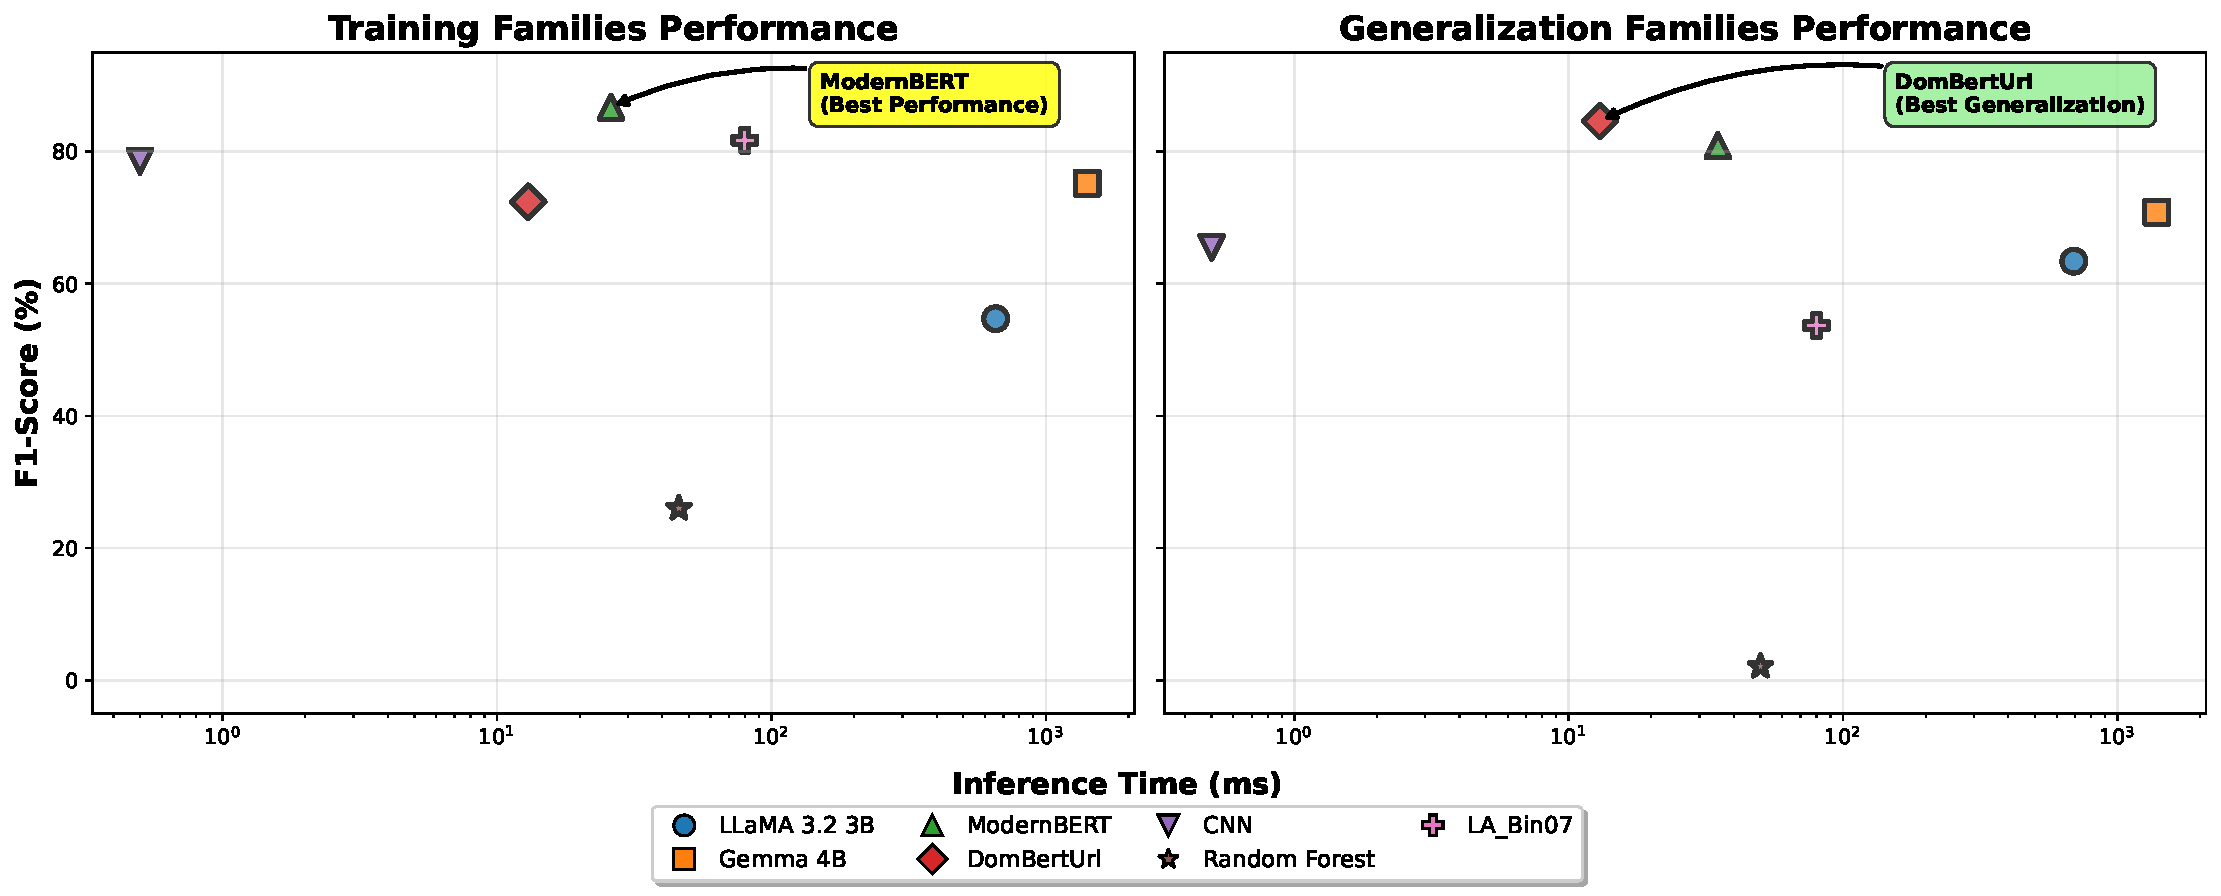
\includegraphics[width=1.0\textwidth]{performance_comparison.pdf}
\caption{Trade-off between F1-score and inference time across training (left) and generalization (right) families. Each point represents one model. ModernBERT stands out with high accuracy and low latency, while DomBertUrl shows strong generalization. The logarithmic time scale highlights large differences in model efficiency.}
\label{fig:performance_comparison}
\end{figure}

We highlight three key findings from these results:

\textbf{1. ModernBERT as the best training model:} As shown in Figure~\ref{fig:performance_comparison}, ModernBERT achieves the highest F1-score on training families (86.7\%) with very low inference time (26ms). This combination of speed and accuracy makes it highly suitable for real-time detection in high-throughput environments.

\textbf{2. DomBertUrl excels in generalization:} Unlike most models that lose performance on unseen families, DomBertUrl improves its F1-score from 72.4\% (training) to 84.6\% (generalization). This rare behavior is likely due to its domain-specific pretraining, making it especially effective against new or unknown wordlist-based DGAs.

\textbf{3. Efficiency differences are critical:} Inference times vary widely—from less than 1ms for CNN to over 1.4 seconds for Gemma. This highlights the importance of efficiency when choosing a model for deployment.

\subsection{Family-Specific Performance Patterns}

To better understand model specialization, we analyze performance at the individual family level. Table~\ref{tab:family-performance} shows the F1-scores for each DGA family.

\begin{table}[ht]
\centering
\caption{F1-score matrix across DGA families. Training families are used for model development, while generalization families assess cross-family robustness. The last row shows F1-score variation from training to generalization (positive means improvement).}
\label{tab:family-performance}
\resizebox{\textwidth}{!}{%
\begin{tabular}{l|c|c|c|c|c|c|c}
\toprule
\textbf{DGA Family} & \textbf{LLaMA} & \textbf{Gemma} & \textbf{ModernBERT} & \textbf{DomBertUrl} & \textbf{LA\_Bin07} & \textbf{CNN} & \textbf{RF} \\
\midrule
\multicolumn{8}{c}{\cellcolor{gray!20}\textit{Training Families}} \\
charbot & 53.2 & 68.3 & \textbf{88.6} & 66.0 & 83.0 & 79.3 & 0.2 \\
deception & 82.8 & \textbf{97.9} & 95.7 & 92.8 & 94.4 & 92.5 & 91.5 \\
gozi & 58.6 & 81.1 & \textbf{90.4} & 63.6 & 84.1 & 79.6 & 0.0 \\
\rowcolor{red!20}
manuelita & 34.5 & 29.7 & \textbf{43.1} & 24.5 & 23.8 & 22.6 & 4.3 \\
matsnu & 83.4 & 90.7 & \textbf{95.2} & 89.5 & 93.0 & 90.1 & 70.4 \\
nymaim & 33.6 & 55.1 & \textbf{89.8} & 62.5 & 87.7 & 81.9 & 25.5 \\
rovnix & 40.7 & \textbf{96.4} & 95.5 & 92.4 & 93.6 & 92.4 & 0.0 \\
suppobox & 51.4 & 82.1 & \textbf{95.2} & 87.8 & 94.2 & 92.9 & 15.7 \\
\midrule
\multicolumn{8}{c}{\cellcolor{gray!20}\textit{Generalization Families}} \\
bigviktor & 71.7 & 40.2 & 77.2 & \textbf{79.0} & 35.6 & 47.3 & 4.2 \\
ngioweb & 81.5 & \textbf{88.6} & 71.8 & 82.6 & 42.0 & 57.7 & 0.0 \\
pizd & 36.9 & 83.5 & \textbf{93.8} & 92.4 & 83.4 & 91.4 & 2.0 \\
\midrule
\textbf{Avg (Train)} & 54.7 & 75.2 & \textbf{86.7} & 72.4 & 81.7 & 78.9 & 26.0 \\
\textbf{Avg (Gen)} & 63.4 & 70.8 & 80.9 & \textbf{84.6} & 53.7 & 65.5 & 2.1 \\
\textbf{Degradation} & \cellcolor{green!20}+8.7 & \cellcolor{red!20}-4.4 & \cellcolor{red!20}-5.8 & \cellcolor{green!20}+12.2 & \cellcolor{red!20}-28.0 & \cellcolor{red!20}-13.4 & \cellcolor{red!20}-23.9 \\
\bottomrule
\end{tabular}%
}
\end{table}

ModernBERT shows the most consistent high performance across training families. DomBertUrl, in contrast, achieves the best results on unseen families, confirming its strong generalization. The manuelita family stands out as particularly difficult for all models, indicating a need for more advanced detection strategies.

\subsection{Expert Selection for MoE Deployment}

The main objective of this study is to select a single expert model for wordlist-based DGA detection within an MoE architecture—not to assign multiple experts to different tasks.

To make this selection, we use the composite score defined in Equation~(2), which combines F1-score, precision, recall, false positive rate, and inference time into a unified metric. As shown in Table~\ref{tab:individual-performance}, this score offers a balanced view of each model’s strengths and weaknesses.

\textbf{ModernBERT} achieves the highest score in training (0.894) and remains strong in generalization (0.851), with an inference time of only 26ms. It combines accuracy, generalization, and speed better than any other model. While DomBertUrl achieves a slightly higher generalization F1 (84.6\%) and a strong score (0.863), it lags behind in training and is less consistent overall.

CNN, although extremely fast ($<$1ms), sacrifices too much accuracy to be suitable for detecting complex DGA patterns.

Based on these results, we select \textbf{ModernBERT as the optimal specialized expert} for wordlist-based DGA detection. Its high accuracy, strong generalization, and low latency make it ideal for real-world deployment in MoE-based cybersecurity systems.


\subsection{Specialization vs. Generalization: Expert Focus vs. Broad Training}

To validate the effectiveness of expert specialization within MoE architectures, we conduct a comparative evaluation between our wordlist-focused expert (ModernBERT) and a generalist version trained on 54 diverse DGA families (ModernBERT\_54F). This comparison directly addresses a fundamental question in MoE deployment: whether specialized experts outperform generalist models with broader training exposure on domain-specific tasks.

The generalist model (ModernBERT\_54F) was trained using the same architecture and hyperparameters as our specialized expert, with the only difference being the training data composition 8 wordlist-based families versus 54 families spanning multiple DGA generation strategies including algorithmic, hash-based, and hybrid approaches. Table \ref{tab:specialization_comparison} and Figure \ref{fig:performance_comparison} present the comparative analysis.

\begin{table}[htbp]
\centering
\caption{Performance comparison between specialized wordlist expert (ModernBERT) and generalist multi-family model (ModernBERT\_54F). The specialized expert demonstrates superior performance on both training and generalization sets, with particularly notable improvements in generalization capability. F1-scores represent averages across respective family sets.}
\label{tab:specialization_comparison}
\begin{tabular}{l|c|c|c}
\toprule
\textbf{Evaluation Set} & \textbf{ModernBERT} & \textbf{ModernBERT\_54F} & \textbf{Improvement} \\
\midrule
Training Families (F1) & 86.7\% & 79.2\% & +8.6\% \\
Generalization Families (F1) & 80.9\% & 62.1\% & +23.2\% \\
\bottomrule
\end{tabular}
\end{table}

\begin{figure}[ht]
\centering
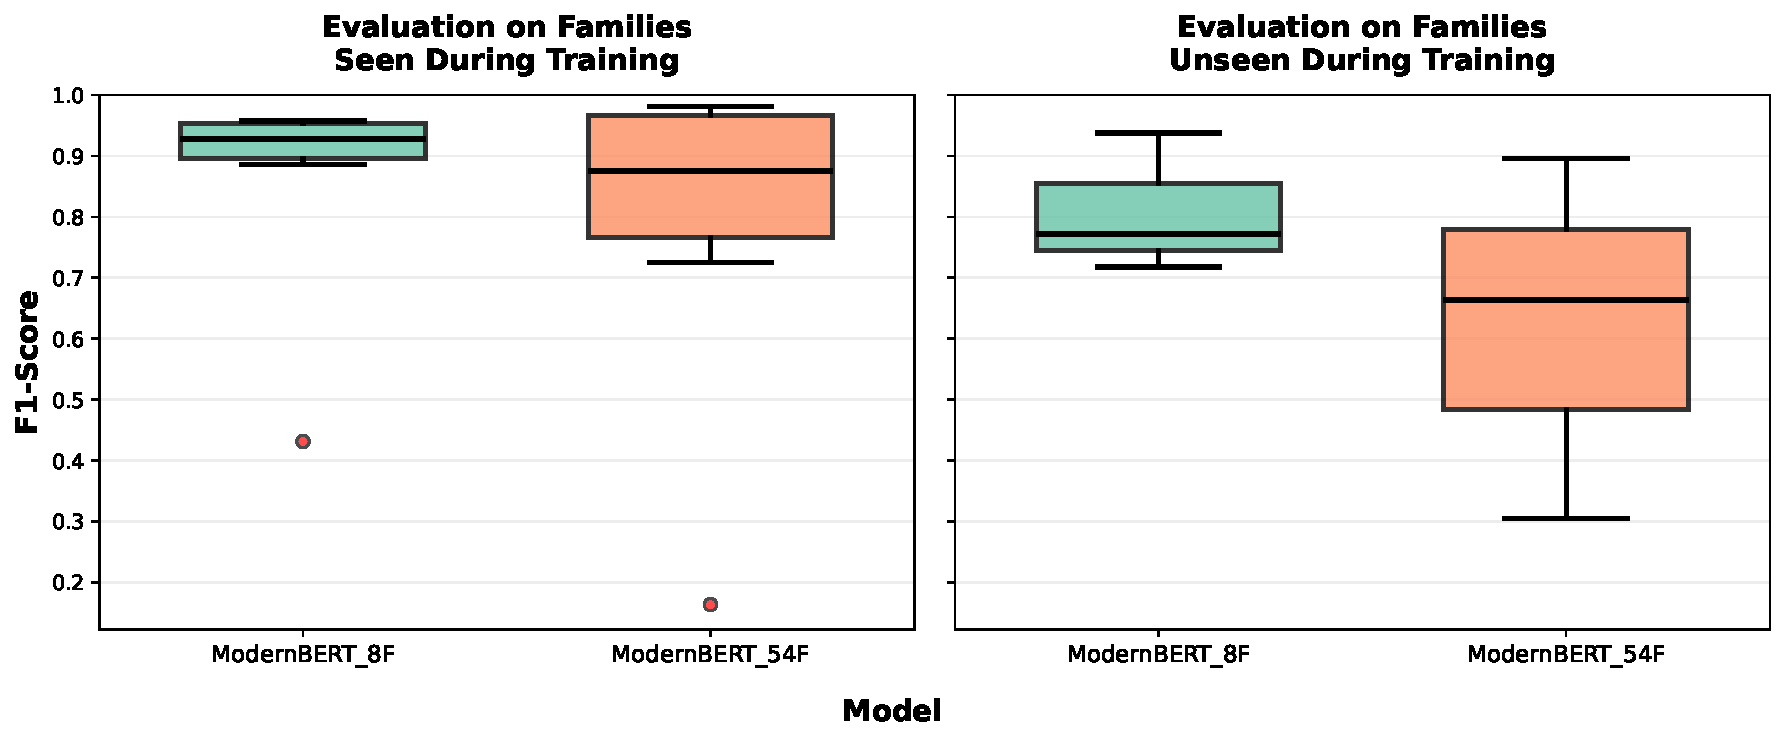
\includegraphics[width=1.0\textwidth]{comparison.pdf}
\caption{F1-Score comparison between specialized wordlist expert (ModernBERT) and generalist model (ModernBERT\_54F) across training families (left) and generalization families (right). The specialized expert consistently outperforms the generalist approach, with particularly pronounced advantages on unseen families. Box plots show median (central line), quartiles (box boundaries), range (whiskers), and outliers (red dots). The superior performance of the specialized model validates the core principle of expert specialization in MoE architectures.}
\label{fig:performance_comparison}
\end{figure}

The results reveal compelling evidence for expert specialization:

\textbf{Training Family Performance:} The specialized expert (ModernBERT) achieves superior performance on wordlist-based families with an average F1-score of 86.7\%, compared to 79.2\% for the generalist model (ModernBERT\_54F). This 8.6\% improvement demonstrates the benefit of focused training on semantically coherent domain generation patterns, validating the hypothesis that specialized models develop deeper understanding of domain-specific characteristics.

\textbf{Exceptional Generalization Advantages:} Most remarkably, the specialized expert shows a dramatic 23.2\% improvement in generalization performance (80.9\% vs. 62.1\%). This counterintuitive finding where focused training leads to better generalization suggests that deep understanding of wordlist-based generation principles enables superior detection of novel variants within the same semantic domain.

\textbf{Robustness Across Difficulty Levels:} Figure \ref{fig:performance_comparison} illustrates that the specialized expert maintains consistent superiority across the performance distribution. The generalist model shows higher variance and more outliers, indicating less reliable performance, while the specialized expert demonstrates more stable and predictable behavior.



These findings provide strong empirical support for the MoE paradigm in cybersecurity applications. Specialized experts not only outperform generalist approaches within their target domain but also demonstrate superior adaptability to emerging threats within that domain. This validates the core MoE principle that focused expertise, rather than broad exposure, is optimal for handling domain-specific challenges in production environments.

\section{Discussion}
\label{sec:discussion}

\subsection{Expert Model Selection Rationale}

The experimental results provide strong support for selecting \textbf{ModernBERT} as the specialized expert for wordlist-based DGA detection within a MoE framework. Several factors contribute to this conclusion:

\textbf{Robust Detection Performance:} ModernBERT consistently achieves top-tier results across training families and maintains high performance on unseen families. It excels on particularly challenging families such as \textit{charbot} (88.6\%), \textit{gozi} (90.4\%), and \textit{nymaim} (89.8\%), reflecting strong pattern recognition. Its balance between recall (86.6\%) and precision (89.7\%) on training data indicates reliable detection with minimal false positives.

\textbf{High Efficiency:} With an inference time of only 26ms, ModernBERT offers a substantial speed advantage over LLaMA (656ms) and Gemma (1413ms), enabling real-time processing even in high-throughput environments. This level of efficiency translates into practical scalability for production systems.

\textbf{Stable Generalization:} Although some performance drop is expected when facing novel threats, ModernBERT’s F1-score decreases modestly from 86.7\% (training) to 80.9\% (generalization), demonstrating solid generalization across unseen wordlist-based DGA families.

\subsection{Insights on Model Behavior}

\textbf{Limitations of Large Language Models:} While LLaMA and Gemma deliver strong precision, their performance is inconsistent across families and their computational costs are significantly higher. These models are unsuitable for real-time deployment scenarios due to their latency and resource demands.

\textbf{Impact of Domain-Specific Pretraining:} DomBertUrl’s impressive generalization performance (84.6\% F1) highlights the benefits of training on domain-related data. Its performance suggests that targeted pretraining can enhance robustness to unseen DGA variants, even when overall capacity is lower than in large-scale language models.

\textbf{Relevance of Lightweight Models:} CNN, despite lower accuracy, offers exceptional speed (sub-millisecond inference), making it suitable for constrained environments or for use as a fallback or filtering layer when ultra-fast response is needed.

\subsection{Challenging Detection Cases}

One of the most striking observations is the consistently poor performance across all models on the \textit{manuelita} family, with the highest F1-score reaching only 43.1\%. Qualitative inspection of this family reveals sophisticated evasion techniques:

\begin{itemize}
\item Use of linguistically coherent domain names with natural syntax and semantics.
\item Inclusion of contextually meaningful word sequences that mimic legitimate usage.
\item Character-level composition designed to evade entropy or rule-based filters.
\end{itemize}

This suggests that even advanced models may require additional signals—such as contextual traffic data or WHOIS metadata—to handle highly evasive families. It also reinforces the need for ongoing evaluation and adaptation in production systems.

\subsection{Deployment Implications}

Selecting ModernBERT as the specialized expert model offers several operational benefits for real-world MoE deployment:

\textbf{Scalability:} Its low latency supports real-time inference across millions of DNS queries per hour, improving system responsiveness without overwhelming resources.

\textbf{Cost and Energy Efficiency:} The efficient runtime reduces infrastructure demands and enables deployment in edge environments or on cost-sensitive platforms.

\textbf{Maintenance Simplicity:} ModernBERT’s consistent performance across families reduces the need for frequent retraining or manual tuning, simplifying system upkeep.



\subsection{Limitations and Future Directions}

Despite strong results, several limitations should be acknowledged:

\textbf{Focus on Expert Selection:} We evaluate models independently rather than implementing a full MoE architecture with routing and decision fusion. Future work should explore integration strategies and their effect on system-level performance.

\textbf{Dataset Scope and Recency:} Although diverse, the dataset may not capture the full spectrum of modern DGA behaviors or the rapid evolution of evasion techniques. Continuous dataset updates are essential for long-term effectiveness.

\textbf{Adversarial Adaptation:} Attackers may adapt to detection mechanisms over time. Exploring adversarial robustness and proactive model hardening is a crucial next step.

\textbf{Generality Beyond Wordlist DGAs:} This study focuses on wordlist-based DGAs. Extending the evaluation to other DGA types (e.g., algorithmic, hybrid, neural) is necessary to generalize the expert selection methodology to broader use cases.


\section{Conclusion and Future Work}
\label{sec:conclusion}

This study provides comprehensive empirical evidence supporting the use of specialized expert selection in MoE architectures for the detection of wordlist-based DGAs—an underexplored but highly evasive DGA category. Through a systematic evaluation of seven diverse models across 11 DGA families, we show that \textbf{ModernBERT} strikes the best trade-off between detection accuracy and computational efficiency for deployment in realistic environments.

In response to recent meta-analyses in the field \cite{cebere2024down}, our methodology explicitly avoids common pitfalls such as overreliance on easy-to-detect DGA families, unrealistic evaluation settings, or closed-source code. By releasing all models, datasets, and evaluation scripts, we enable full reproducibility and facilitate meaningful comparison for future research.

Our main findings include:
\begin{enumerate}
    \item Transformer-based models tailored for short-text input outperform both traditional models and general-purpose language models on wordlist-based DGAs.
    \item Efficiency is not a secondary concern: models must meet latency and resource constraints to be deployable at scale.
    \item Per-family variability in detection accuracy suggests a strong case for modular architectures like MoE, where experts specialize in distinct DGA characteristics.
    \item Classical models still offer value in highly constrained scenarios where resources are extremely limited.
\end{enumerate}

\textbf{Future Work Directions:}
\begin{itemize}
    \item \textbf{Complete MoE Implementation:} Build and evaluate a full MoE system with dynamic routing, expert coordination, and adaptive fallback mechanisms across DGA categories.
    
    \item \textbf{Advanced Robustness Techniques:} Integrate ensemble learning, adversarial training, and contextual features (e.g., DNS response patterns) to improve performance on stealthy or evasive DGA families like \textit{manuelita}.
    
    \item \textbf{Feedback-Driven Routing:} Explore adaptive gating networks that incorporate real-world feedback (e.g., false positives, telemetry) to refine expert selection dynamically.
    
    \item \textbf{Cross-Domain Evaluation:} Extend our expert selection framework to non-DGA tasks, such as phishing domain detection or malicious subdomain identification, to validate its generalizability.
    
    \item \textbf{Operational Deployment Studies:} Conduct long-term evaluations in live network environments to test robustness under traffic variability, concept drift, and emerging DGA strategies.
\end{itemize}

Our results demonstrate that principled expert selection—grounded in realistic assumptions and reproducible evaluation—can enable practical and effective DGA detection. This lays the groundwork for a new generation of modular, adaptive, and scalable cybersecurity systems capable of meeting the demands of modern threat landscapes.


\bibliographystyle{splncs04}
\bibliography{cas-refs}



\end{document}






